% 
%  chapter6.tex
%
\chapter{Evaluation}~\label{ch:eval}
In this chapter, the evaluation and testing methodology of each module that make up CASCIFFO are detailed.
The chapter has the following structure:
\begin{enumerate}
    \item General Requirements Validation;
    \item Meeting the Functional Requirements;
    \item Integration Tests Environment.
\end{enumerate}

\section{General Requirements Validation}~\label{ch:eval:sec:reqs}
In this section the level of fulfillment of each general requirement, as they were specified, is analyzed.

It is structured as follows:
\begin{itemize}
    \item Visualization and management of Clinical Trials as a process;
    \item Ability to edit and validate data (edit checks);
    \item Access control based on different user profiles;
    \item Access by computer, tablet or smartphone;
    \item Ability to export information in numerical or graphical mode;
    \item Ability to customize the form of visualization;
    \item Non-Functional requirements.
\end{itemize}


\subsection{Visualization and management of Clinical Trials as a process}
The visualization of clinical trials is split in two divisions between the proposal of clinical trials and active clinical trials. These two divisions are then split between the general and detailed view. The former showcases the data in a tabular manner, following in the mock-UI, while in detailed view we can view and manage the process of validation described in processes section.

Having said this, this requirement has been completely fulfilled.

\subsection{Ability to edit and validate data (edit checks)}
The ability to edit and validate data is available within the detailed view of proposals and/or clinical trials. In addition, the clinical trials also displays information on scheduled monitoring visits of their participants, which also provides a way of editing their respective data.

Onto validation, which is especially prevalent in the scope of a proposal's process when it comes to validating the financial contract or the protocol of a clinical trial proposal. These validations can be made by adding a mandatory observation along with the state of the validation.

To conclude, this requirement has been fulfilled.

\subsection{Access control based on different user profiles}

To introduce access control, several roles were introduced in the platform, these roles play a part in the validation process of clinical trials, for example, only users with the role of financial and juridical department can validate the financial contract of a proposal submission. 
Besides data checks and validation, some screens also require a certain role to be viewed, for example, only the super user role can view the data management screens.

To finalize this requirement can be considered as fulfilled.

\subsection{Access by computer, tablet or smartphone}

With the goal in mind of CASCIFFO being able to be accessed by any device, mobile or desktop, the platform was developed to be a \acrshort{pwa} along with being a reactive application, rearranging its content to fit appropriately based on the device's screen proportions. 

Although the \acrshort{pwa} feature was not included in the final version of the platform, due to the apache hosting being via HTTP instead of HTTPS (a requirement of a \acrshort{pwa}). The platform can be accessed by any device with any modern web browser. As such, this requirement has been fulfilled.

\subsection{Ability to export information in numerical or graphical mode}
The platform offers the possibility of exporting tabular data into Excel files. The exported data will contain a row per line with each column separated by commas.

This requirement was fully achieved as it was specified.


\subsection{Ability to customize the form of visualization}

Throughout the several screens in CASCIFFO, data is displayed mainly through data tables and graphical data, the ability to customize the form of visualization, as specified in the functional requirements analysis, is represented by the ability to filter tables as for them to display only necessary information.

This requirement has been fulfilled.


\subsection{Non-functional requirements}

Both the optional and mandatory have been implemented with the exception of point 4, which was not possible due to data regulations issues that prevented the integration with the \acrshort{hff}'s "Admission" database.


\section{Meeting the Functional Requirements}~\label{ch:eval:sec:meeting-reqs}
According to the functional requirements the screens were developed based on the mock ups detailed in the report.  The developed dashboard screen displays several useful stats through graphs and tables.

Each page corresponds to a route that is handled by \textit{React.Router} as mentioned previously in the document.
Most of the requirements were fulfilled exactly as detailed in the mock-ups, as such, here we will focus on the ones that ended up with significant differences and additional screens that weren't in the requirements, namely:

\begin{itemize}
    \item The addition of the financial contract tab when viewing the details of a clinical trial proposal;
    \item A user management page accessible only by the admin;
    \item Data management page to delete/create/update several data types, such as service type, therapeutic area and pathology.
    \item The implementation of the dashboard;
\end{itemize}

Along side these main changes, the filter options on general screens such as the proposal and research overview screens were removed due to the ability of filtering by property together with sorting by column.

\subsection{Financial contract tab}

The development of this additional tab, viewed in figure~\ref{fig:cf-tab-ui} was to centralize the validation of the financial contract in one place, since the state where the financial contract awaits validation is a two-step process involving both juridical and financial departments of \acrshort{hff}. The refusal on one's side implicates a new financial contract submission. In addition, this tab also facilitates viewing the history of approvals/refusals.

\begin{figure}[H]
    \centering
    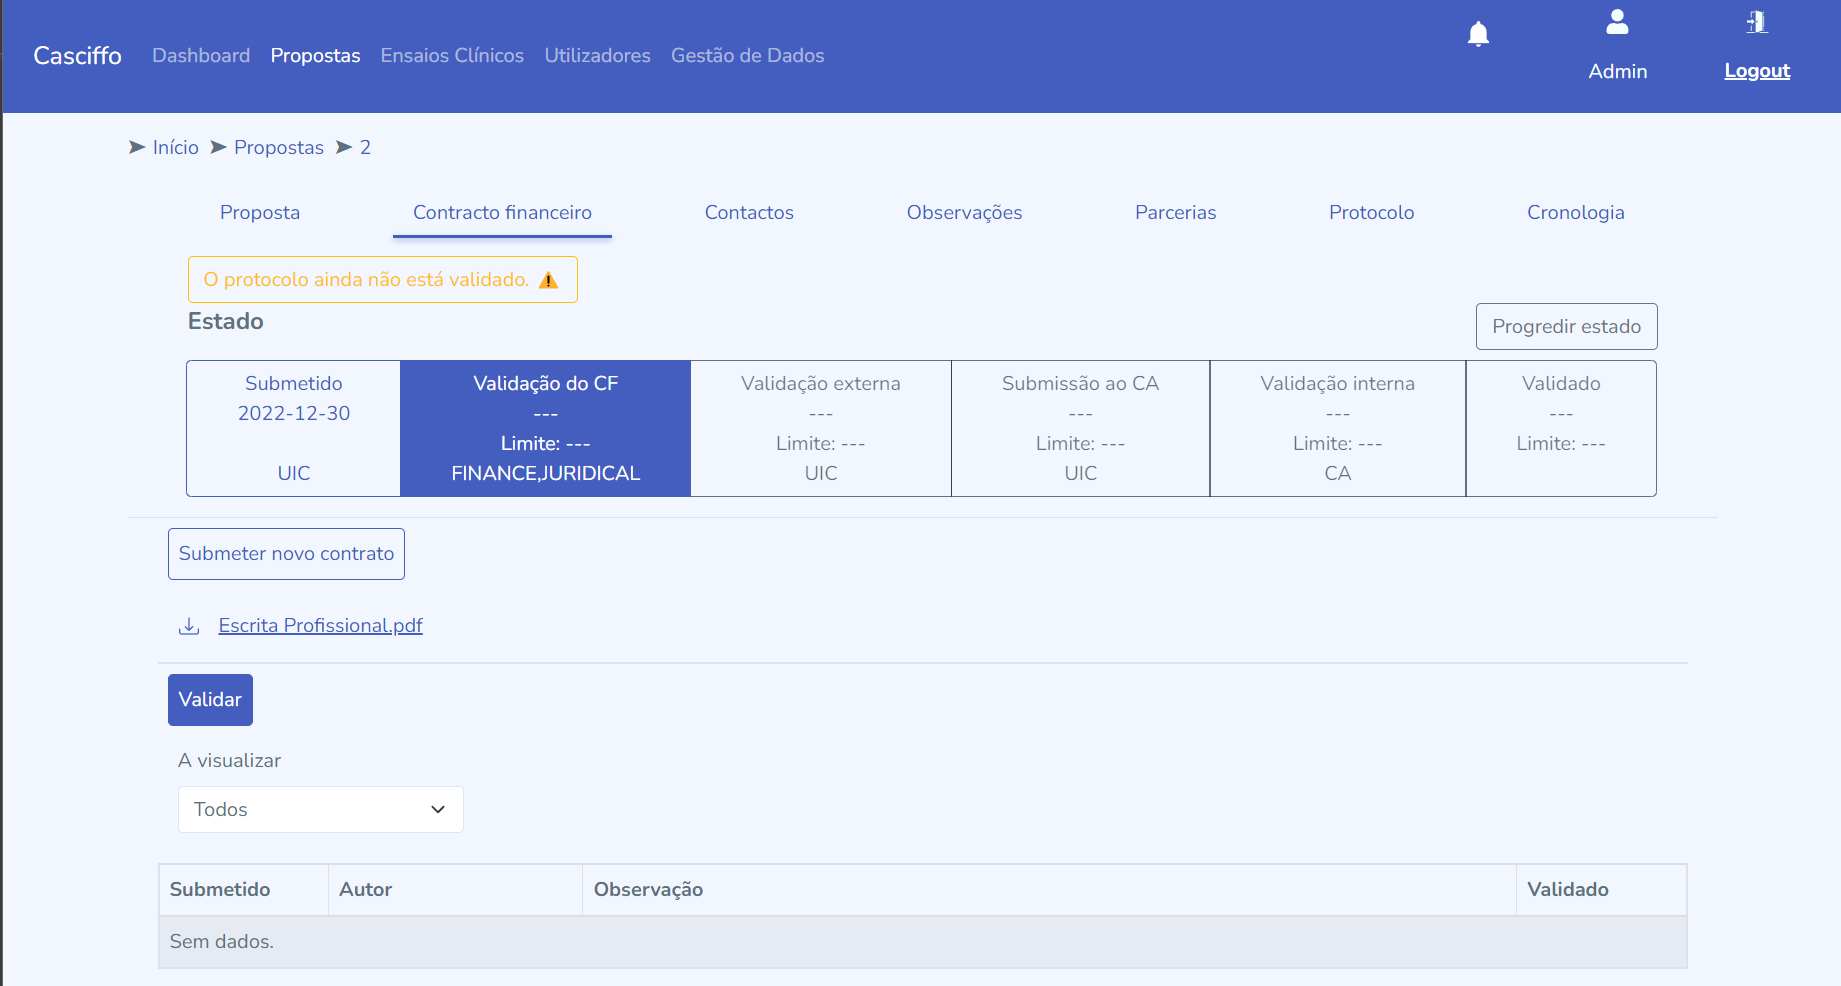
\includegraphics[scale=0.4]{Chapters/img/ui/proposal-cf-tab.png}
    \caption{Financial contract tab UI.}
    \label{fig:cf-tab-ui}
\end{figure}

\subsection{User management page}
Without a defined way of automatically pulling investigator data, this has to be introduced manually, thus the increased need for this screen, viewed in figure~\ref{fig:user-management-ui}, arouse. In this screen, available only to administrator level users, users can be created by defining their name and email, afterwards the user themselves can define their own password. In conjunction with this feature, administrators can also grant and revoke permissions to other users.


\begin{figure}[H]
    \centering
    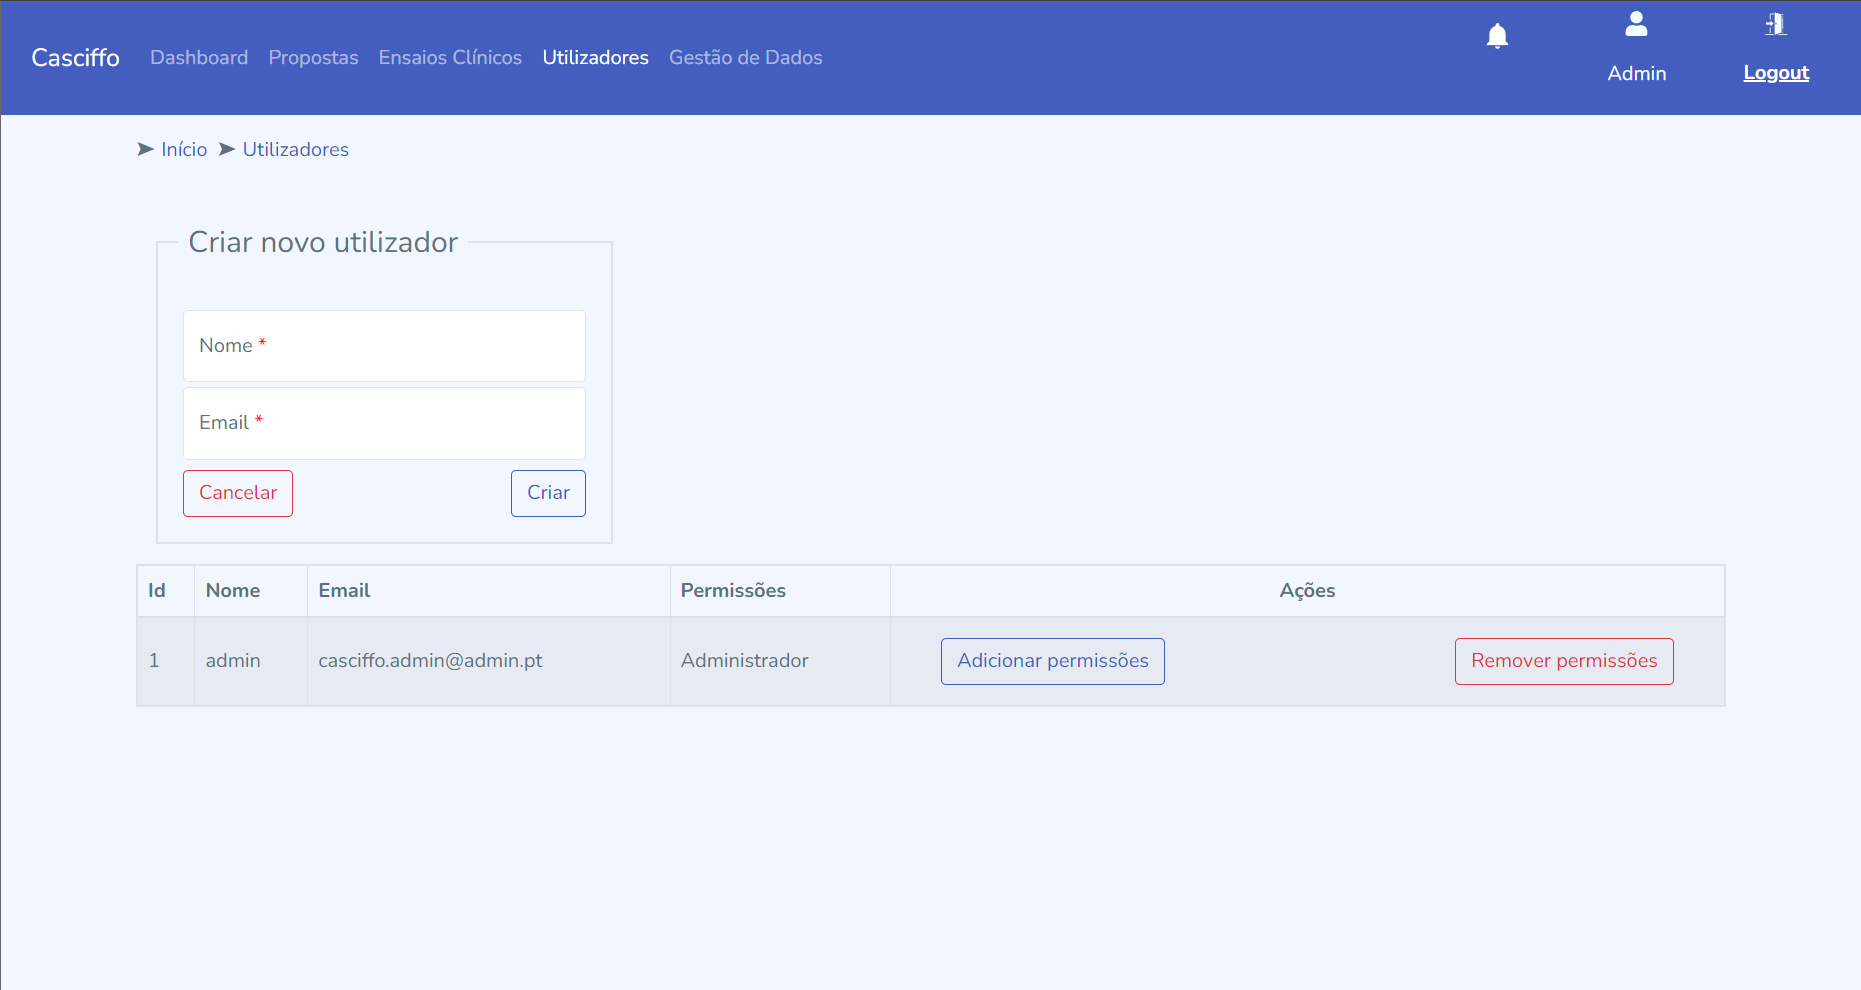
\includegraphics[scale=0.4]{Chapters/img/ui/user-management.png}
    \caption{User Management UI.}
    \label{fig:user-management-ui}
\end{figure}

\subsection{Data management page}
The page of data management, in similarity to the user management page, is only available to administrator level users, allowing the creation, edit and deletion of data that can't otherwise be created normally in the application.
This page, as viewed in figure~\ref{fig:data-management-ui}, is organized by several tabs with their own purpose. The data for service types, therapeutic areas, pathologies, as well as patient data is manually created here.

\begin{figure}[H]
    \centering
    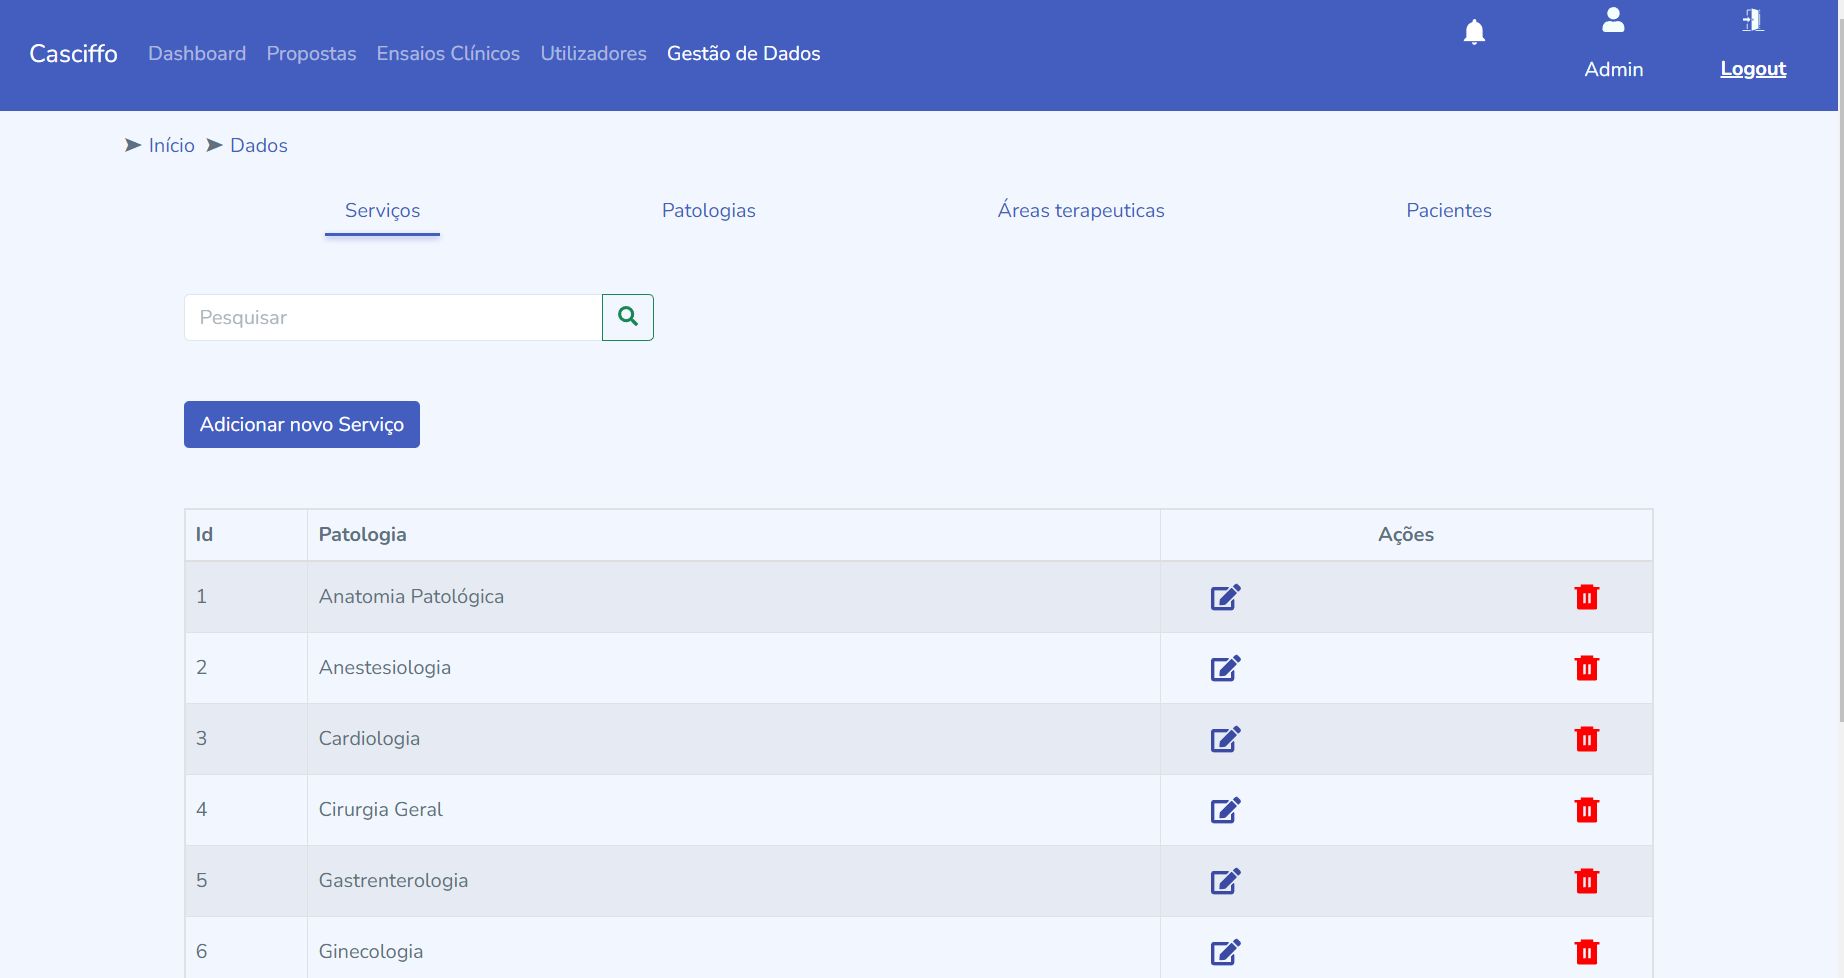
\includegraphics[scale=0.4]{Chapters/img/ui/data-management.png}
    \caption{Data management UI.}
    \label{fig:data-management-ui}
\end{figure}


\subsection{Dashboard}
The development of the dashboard was made with the goal of being able to view relevant data displayed in graphs and tables. Making an observation of this screen as viewed in figure~\ref{fig:dashboard-ui-1}, the data displayed in the first row of graphs refers to the amount of completed, on-going and canceled clinical and observational trials on the left hand side, while on the right hand side the amount of submitted, on-going validation and fully validated proposals is shown.
Moving to the section table data section, the five most recently updated trials and proposals are shown. Below these two tables, the most events occurring on the current week are shown in a tabled manner as well as viewed in the figure~\ref{fig:dashboard-ui-2}.


\begin{figure}[H]
    \centering
    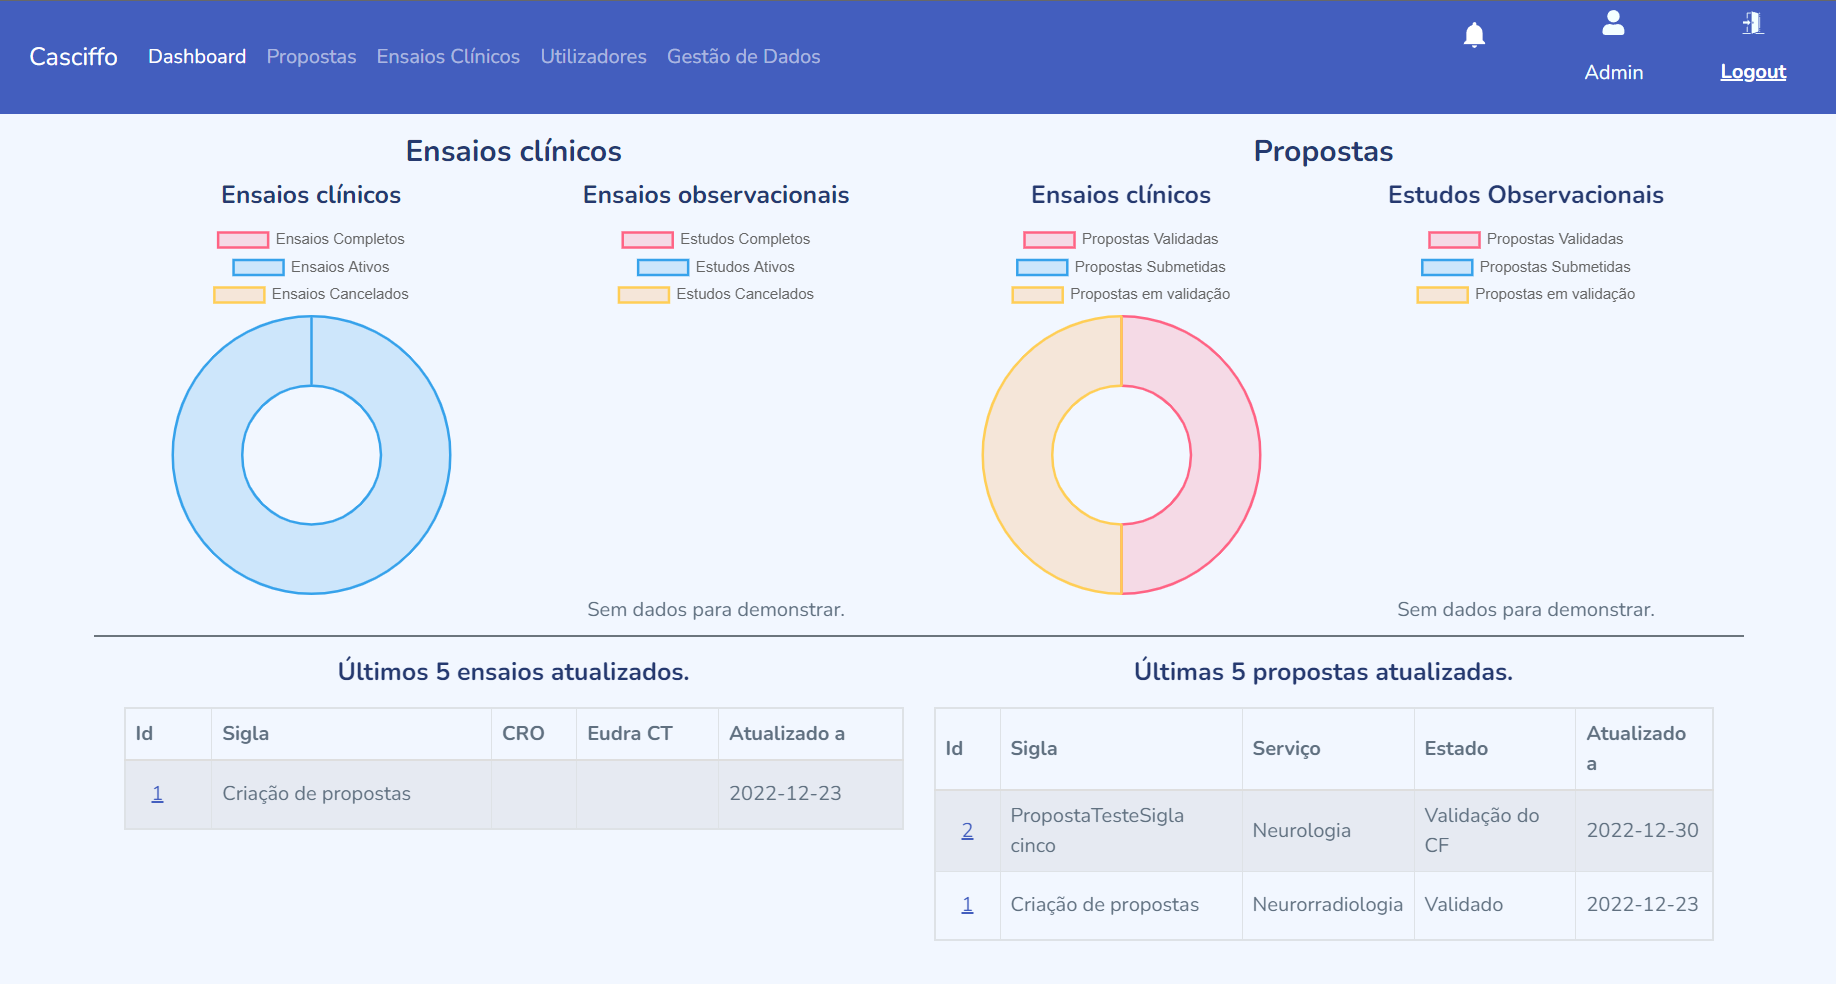
\includegraphics[scale=0.4]{Chapters/img/ui/dashboard-1.png}
    \caption{Dashboard UI 1/2.}
    \label{fig:dashboard-ui-1}
\end{figure}

\begin{figure}[H]
    \centering
    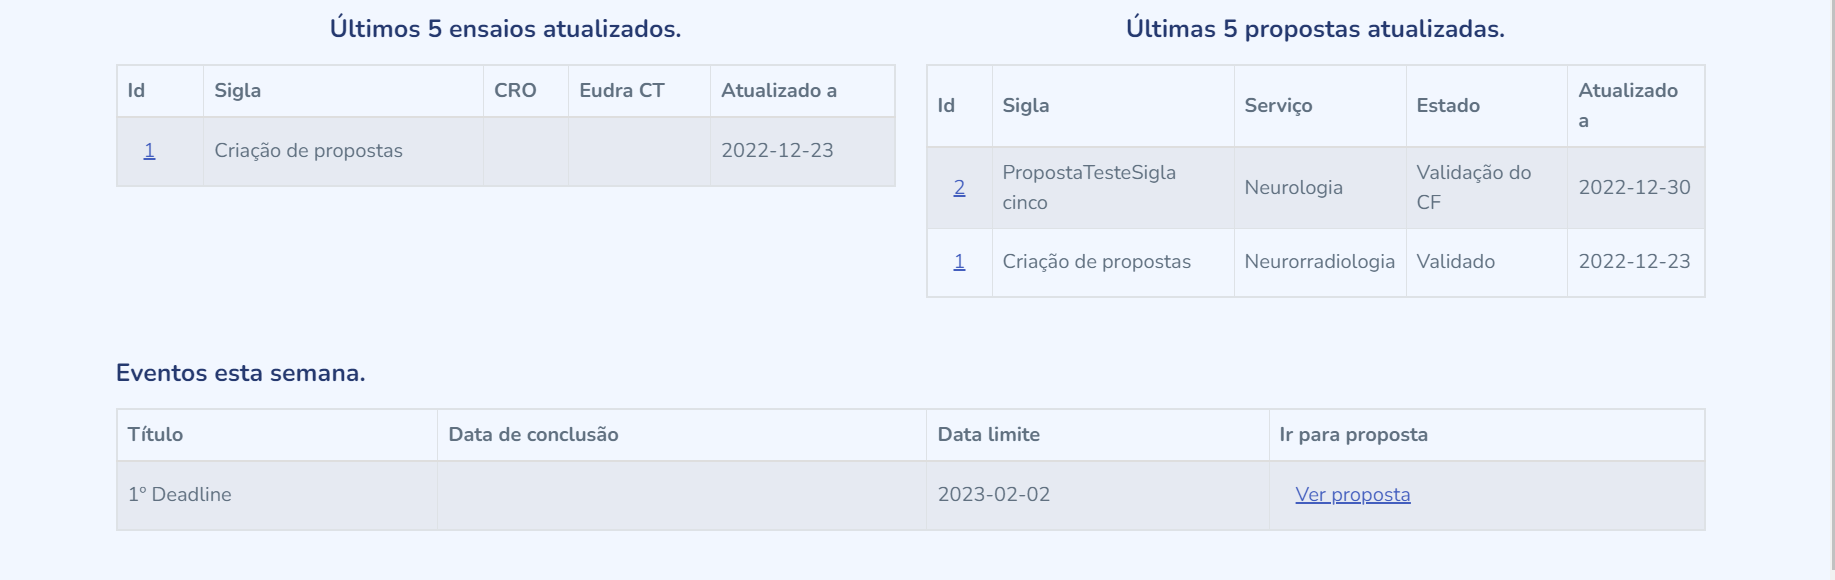
\includegraphics[scale=0.4]{Chapters/img/ui/dashboard-2.png}
    \caption{Dashboard UI 2/2.}
    \label{fig:dashboard-ui-2}
\end{figure}


\section{Integration Tests Environment}\label{ch:eval:sec:integration-tests-env}

The application was tested in two different environments, in the local machine and on a remote server hosted on \textit{Heroku}. 
In the former environment the tests consisted in integration tests to validate the logic of the \acrshort{be} module. 

\subsection{Integration Tests}
The developed integration tests were made to validate each layer of the \acrshort{be} module, from the repository to the service and finally controller layer. To create the integration tests, the \textit{Spring Unit} testing framework, was used in conjunction with the in-memory relation database management system \textit{H2}~\cite{h2-db} so that they could run without affecting the development database. The configurations required to set up this in-memory database require a different set of configurations compared to when using the main database. This can be achieved by creating another \lstinline{.properties} file with its name set to \lstinline{application-test}, thus creating the file \lstinline{application-test.properties}, a snippet of which can be viewed in listing~\ref{lst:spring-h2-config}. The striking differences are apparent in the properties \lstinline{spring.r2dbc.url}, \lstinline{spring.r2dbc.username} and \lstinline{spring.sql.init.data-locations}. The first two are now set to the configurations of the \textit{H2}, while the last one indicates where the testing data is located.

\begin{lstlisting}[
caption={Spring properties configurations with H2 database.},
label={lst:spring-h2-config}
]
# Database settings
spring.r2dbc.url=r2dbc:h2:mem:///~/test;MODE=PostgreSQL;
spring.r2dbc.username=SA
spring.sql.init.schema-locations=classpath:sql/schema.sql
spring.sql.init.data-locations=classpath:sql/data-h2-test.sql
\end{lstlisting}

In addition to the changes of the configuration file, we also require new testing libraries on the project, namely \textit{H2}, \textit{Spring Boot} and coroutines testing libraries. With this goal in mind, the following dependencies in listing~\ref{lst:spring-test-config} were added to the \lstinline{build.gradle.kt} file.

\begin{lstlisting}[
caption={Spring test dependencies snippet.},
label={lst:spring-test-config}
]
dependencies {
    // implementation and runtimeOnly dependencies...
    // test dependencies.
    testImplementation("io.r2dbc:r2dbc-spi:1.0.0.RELEASE")
    testImplementation("com.h2database:h2:2.1.214")
    testImplementation("io.r2dbc:r2dbc-h2:1.0.0.RELEASE")
    testImplementation("org.springframework.boot:spring-boot-starter-test:3.0.0")
    testImplementation("io.projectreactor:reactor-test:3.4.24")
}
testImplementation ("org.jetbrains.kotlinx:kotlinx-coroutines-test:1.6.4")
\end{lstlisting}

In order to start \textit{H2}~\cite{h2-db}, assuming it is installed, the service needs to be launched and afterwards it should automatically open a browser and direct the user to a localhost URL that initially may display an unsafe warning. This warning can be ignored since it is running on the local machine, not remotely. Upon advancing, the user is met with a login screen, here we can configure the credentials according to the previously created configurations, resulting in the settings which can be observed in figure~\ref{fig:h2-login-config}.

\begin{figure}[H]
    \centering
    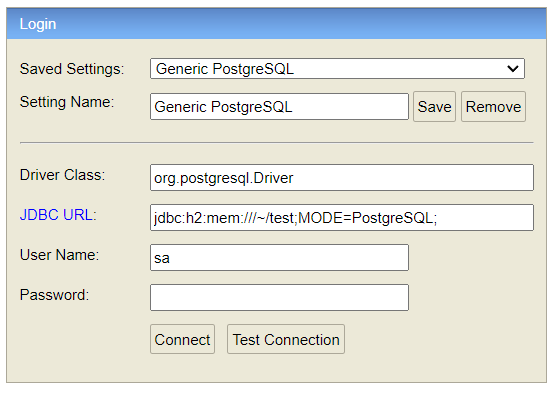
\includegraphics{Chapters/img/misc/h2-login-config.png}[scale=0.5]
    \caption{H2 configurations.}
    \label{fig:h2-login-config}
\end{figure}

With the database created and configured, the next step consists in creating the test classes. In order for these classes to use the different application properties, the annotation \lstinline[keywordstyle=\color{black}]{@ActiveProfiles(value = ["test"])} was be used to declare which Spring profile the application will use when loading the application context for test classes. In addition, to launch the tests with the required application context with Spring Boot and provide other features, the annotation \lstinline{@SpringBootTest} was also used. A test file was created for each component with several methods testing the control flow and logic of their respective component. Since the application environment is non-blocking, two approaches were used to implement the tests. The first consists in using the \lstinline{StepVerifier} utility class, provided in the Project Reactor library that includes utility test methods that assert the behavior of reactive data streams of \lstinline{Mono} and \lstinline{Flux}. This is especially useful for testing the repository component, for example, in the listing~\ref{lst:test-proposal-repo}, we verify the correct verification of a proposal entity. Through several methods available in the utility class \lstinline{StepVerifier}, the entire behavior of the data stream can be tested. It is important to have each \lstinline{StepVerifier} block run the method \lstinline{.expectSubscription()} to subscribe to the stream passed as argument.

\begin{lstlisting} [
language={kt},
caption={Test method for the Proposal Repository.},
label={lst:test-proposal-repo}
]
 @Test
fun whenProposalCreated_thenFindIdInRepository() {
    val proposal = ProposalModel(
        sigla = "Created for test",
        type = ResearchType.OBSERVATIONAL_STUDY,
        stateId = 1,
        principalInvestigatorId = 1,
        therapeuticAreaId = 1,
        serviceTypeId = 1,
        pathologyId = 1
    )

    StepVerifier
        .create(proposalRepository.save(proposal))
        .expectSubscription()
        .`as`("Create proposal")
        .consumeNextWith {
            assert(it.id !== null)
            proposal.id = it.id
        }
        .expectComplete()
        .log()
        .verifyThenAssertThat()

    StepVerifier
        .create(proposalRepository.findById(pId = proposal.id!!))
        .expectSubscription()
        .`as`("Find created proposal with id ${proposal.id}")
        .thenAwait()
        .assertNext {
            it.id === proposal.id
        }
        .expectComplete()
        .log()
        .verifyThenAssertThat()
}   
\end{lstlisting}

This approach was used to test the repository layer, as each repository returned reactive data streams.

The second approach which was used to test the service layer, consisted in realizing the test inside a coroutine with the keyword \lstinline{runBlocking} which runs a coroutine in a blocking manner, meaning that the code inside it will be executed synchronously and will block the current thread until the coroutine completes, an example of this can be observed in listing~\ref{lst:test-add-patient-service}. It is important to note that this approach was used since the service layer heavily relies on \textit{Kotlin coroutines}.

\begin{lstlisting}[
language={kt},
caption={Unit integration test for adding a patient to an on-going research.},
label={lst:test-add-patient-service}
]
@Test
fun testServiceAddPatientToResearch() {
    var patient = PatientModel(
        processId = 102,
        fullName = "Manuel Santos",
        gender = "m",
        age = 50
    )
    runBlocking {
        patient = patientService.save(patient)
        val addedPatient = participantService.addPatientToResearch(patientId = patient.id!!, researchId = 1)
        val patients = patientService.findAllByResearchId(researchId = 1)
        assertDoesNotThrow {
            patients.first { assert(it.id === addedPatient.id) }
        }
    }
}
\end{lstlisting}

Finally the controller layer was tested using an external tool called \textit{Postman}. This platform allows the user to verify the responses and facilitate the ability to manipulate the header requests as well as viewing the response headers. The Postman request collection is available within the \textit{Github} repository.
Within Postman there are several fields we can define to build a request and receive a response, as viewed in the figure~\ref{fig:postman-post-req} which depicts a login request. This is a POST request made to the application running in localhost, hence the localhost URL which is defined with the variable \lstinline{localhost} surrounded by curly braces, along with the request body specifying the credentials of the user. Upon executing the request, the response received is also detailed the figure, consisting of the access token of the user, their roles, user id and user name.

\begin{figure}[H]
    \centering
    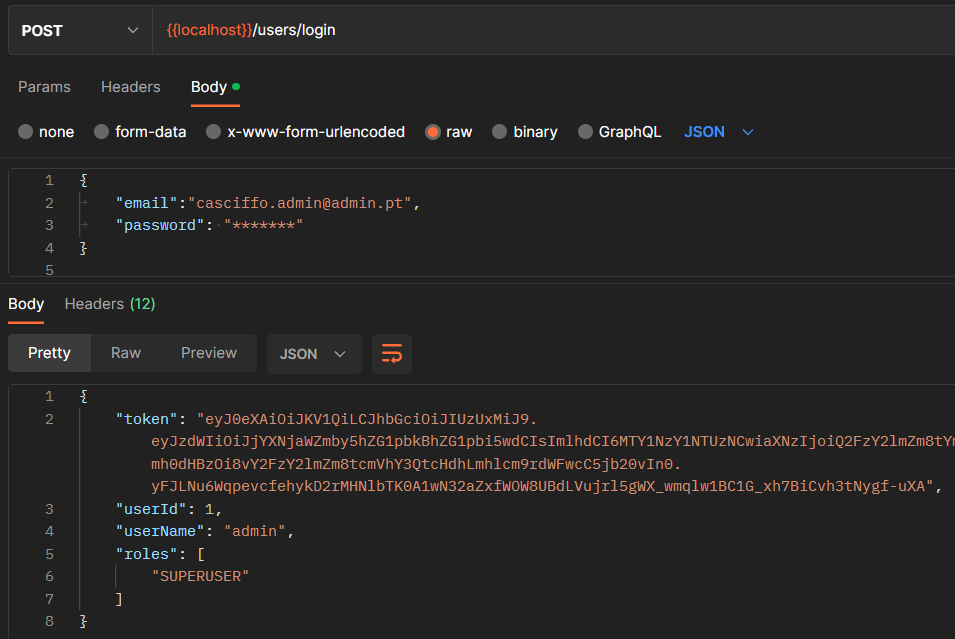
\includegraphics[scale=0.5]{Chapters/img/misc/postman-req-post.png}
    \caption{Authentication request made in Postman.}
    \label{fig:postman-post-req}
\end{figure}

Moving to the \acrshort{fe} module, testing consisted of continuous manual usage with addition of the developer tool \textit{Lighthouse}. \textit{Lighthouse} is an open-source automated tool for improving the quality of web pages by running diagnostic reports on the page. This tool was used on the production build to measure performance, the report can be seen in figure~\ref{fig:lighthouse-report}. The main metrics are Performance, Accessibility, Best Pactices, SEO and compatibility with a \acrshort{pwa}.

\begin{figure}[H]
    \centering
    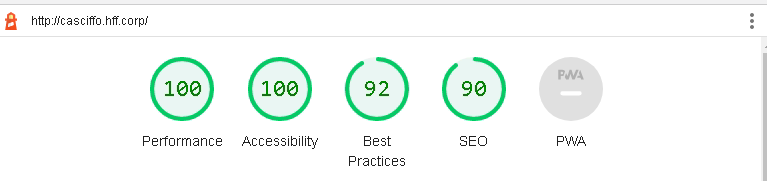
\includegraphics[scale=0.6]{Chapters/img/lighthouse/report-1-no-pwa.png}
    \caption{Lighthouse metrics report.}
    \label{fig:lighthouse-report}
\end{figure}
 
The performance metrics can be seen further into the report, as shown in figure~\ref{fig:lighthouse-pmetrics}.
These metrics are in regard to loading speed performance.

\begin{figure}[H]
    \centering
    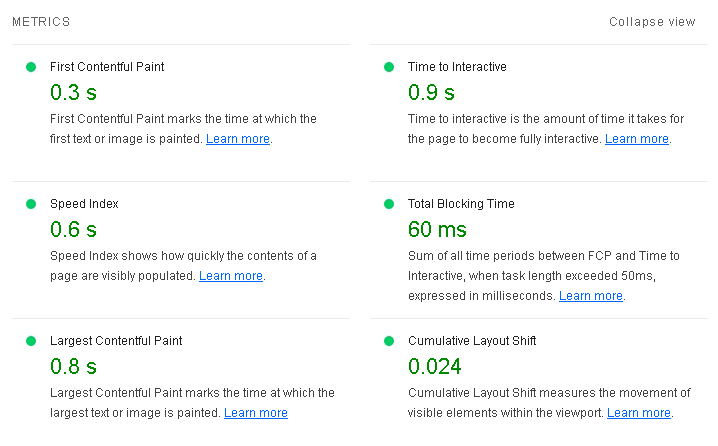
\includegraphics[scale=0.5]{Chapters/img/lighthouse/report-1-no-pwa-metrics.png}
    \caption{Lighthouse performance metrics.}
    \label{fig:lighthouse-pmetrics}
\end{figure}

The \acrshort{pwa} metric is inactive as seen in the lighthouse metrics report because the developed solution does not meet all of the \acrshort{pwa} requirements. Although the platform is fully adapted to be a \acrshort{pwa}, without the requirement of having the application being hosted in HTTPS instead of HTTP, the platform won't be able to take advantage of the \acrshort{pwa} functionality.
Taking a deeper look into the report on the \acrshort{pwa} section (figure~\ref{fig:lighthouse-pwa}), we are warned that no service workers have been registered. Once again, this is because service workers are not allowed to execute when hosted over HTTP connections. Thus, as long as the developed solution is served via HTTP, it cannot be considered a \acrshort{pwa}.

\begin{figure}[H]
    \centering
    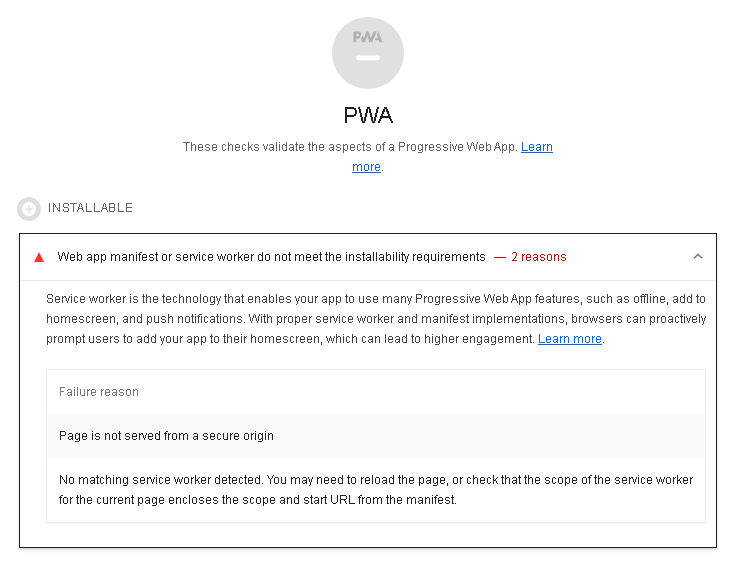
\includegraphics[scale=0.5]{Chapters/img/lighthouse/report-1-rip-pwa.png}
    \caption{Lighthouse PWA section report.}
    \label{fig:lighthouse-pwa}
\end{figure}

\subsection{Heroku Environment}
The testing environment provided by \textit{Heroku} allowed for the methodology of Continuous Integration and Continuous Development, by allocating platform in conjunction with \textit{PostgreSQL} database. This methodology allows for several benefits such as speed, reliability and faster release rate. With the application readily available in \textit{Heroku} we can utilize the application to manually verify user experience and validate the specified requirements for the application.
